\documentclass{article}
\usepackage[utf8]{inputenc}
\usepackage[margin=0.7in]{geometry}
\usepackage{amsmath}
\usepackage{amssymb}
\usepackage{listings}
\usepackage{graphicx}
\usepackage{float}

\graphicspath{{images/}}

\title{Solutions to the Assignment - 2 : CS5480 - \\
Deep Learning}
\author{Vishwak Srinivasan\\
\texttt{CS15BTECH11043}}
\date{}

\begin{document}
\maketitle

\section*{Question 1}
\subsection*{Part a}
\begin{flushleft}
The code for the neural net in available in the file \texttt{Question1.py}. The instructions for running this code can be obtained by running \texttt{python3 Question1.py -h}. Single string help statements have been provided, and default values have been shown.

A check for correctness of the program specified in the problem was to try a full-batch gradient descent algorithm for the loss function. As expected, the loss decreased monotonically. The graph of this variation is shown below:
\begin{figure}[H]
\centering
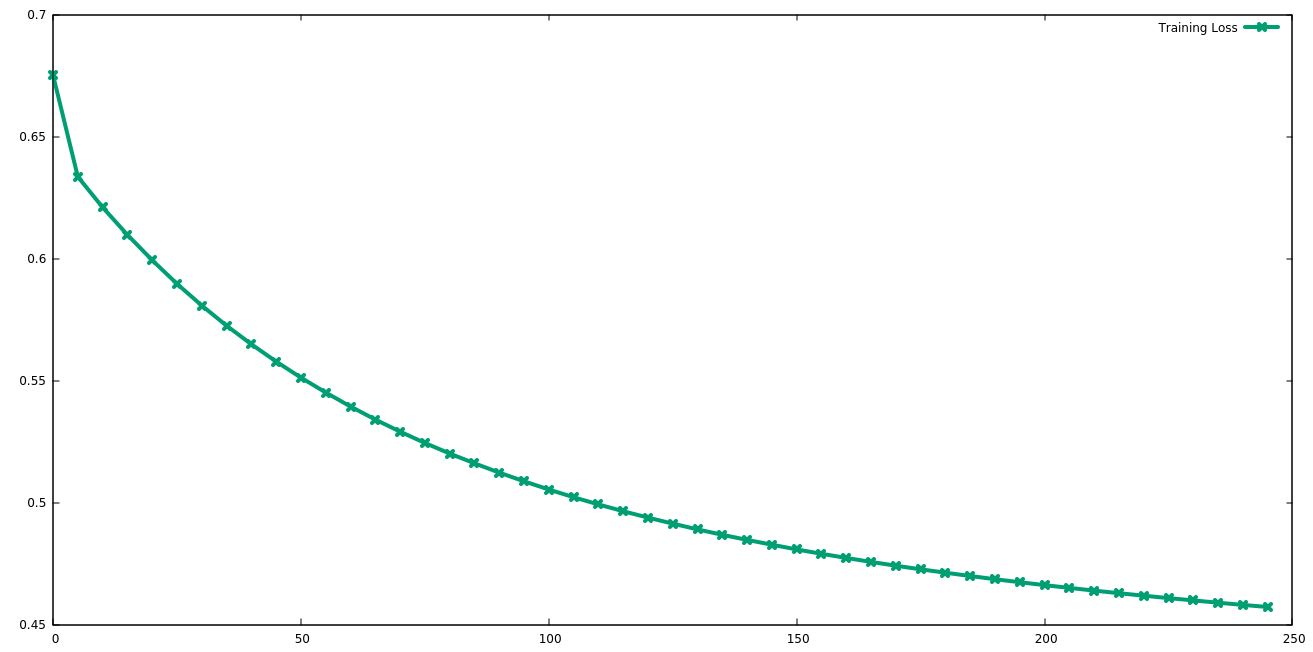
\includegraphics[width=0.7\linewidth]{train_full_batch_q1.png}
\end{figure}
\end{flushleft}

\subsection*{Part b}
\begin{flushleft}
This baseline accuracy is implemented in the results section of the code. To make an proper random guess, it is important to know the class-(im)balance in the output labels. I calculate these probabilities and create a tensor of the length of the targets and initialize using \texttt{torch.bernoulli(p=<calculated probability>)}. Lines of interest in the script are L169-L178 and L192-L201.
\end{flushleft}

\subsection*{Part c}
\begin{flushleft}
I used a constant learning rate schedule. For the specifications of this problem i.e., \texttt{batch\_size} = 100, \texttt{H} = 5, the best learning rate I could get is 0.008 (chosen from a set \(\{0.0001, \ldots, 0.0009, 0.001, \ldots, 0.009, 0.01, \ldots, 0.05 \}\)). The random state is saved in \texttt{random-state.pt} for reproducibility. I trained it until the training classification error increased considerably per epoch (``jumping from an otherwise stable point") or didn't decrease considerably per epoch (reaching a ``local minimum"), which in this case was 96 epochs. The training set accuracy achieved after 96 epochs was \(92.91\%\) and the testing set accuracy achieved after 96 epochs was \(93.99\%\). Below are the graphs of the variations observed (L: Train, R: Test):
\begin{figure}[H]
\begin{minipage}{0.49\linewidth}
\centering
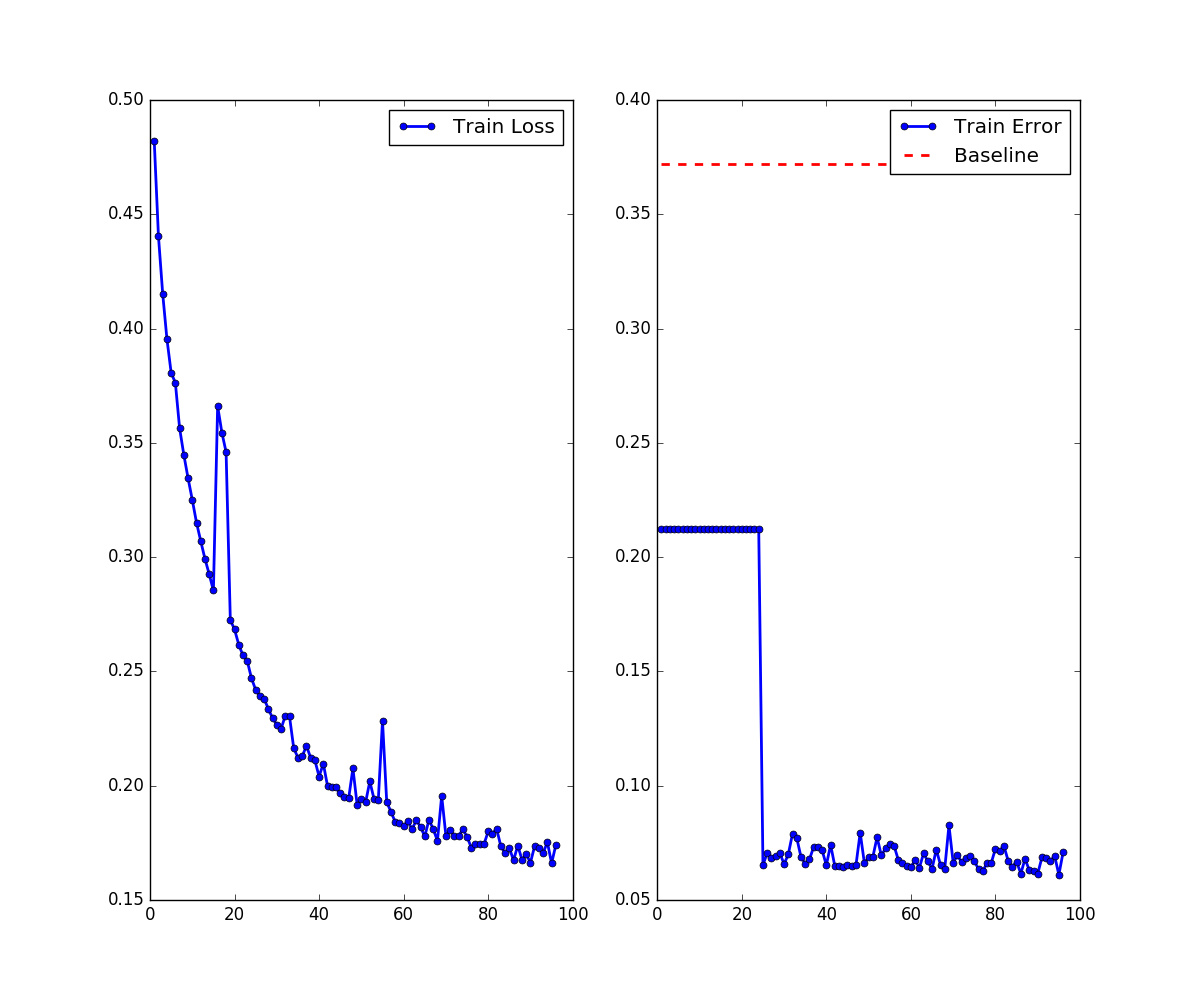
\includegraphics[width=0.95\textwidth]{Train-Statistics-sgd-batchsize=100-bce.png}
\end{minipage}
\hfill
\begin{minipage}{0.49\linewidth}
\centering
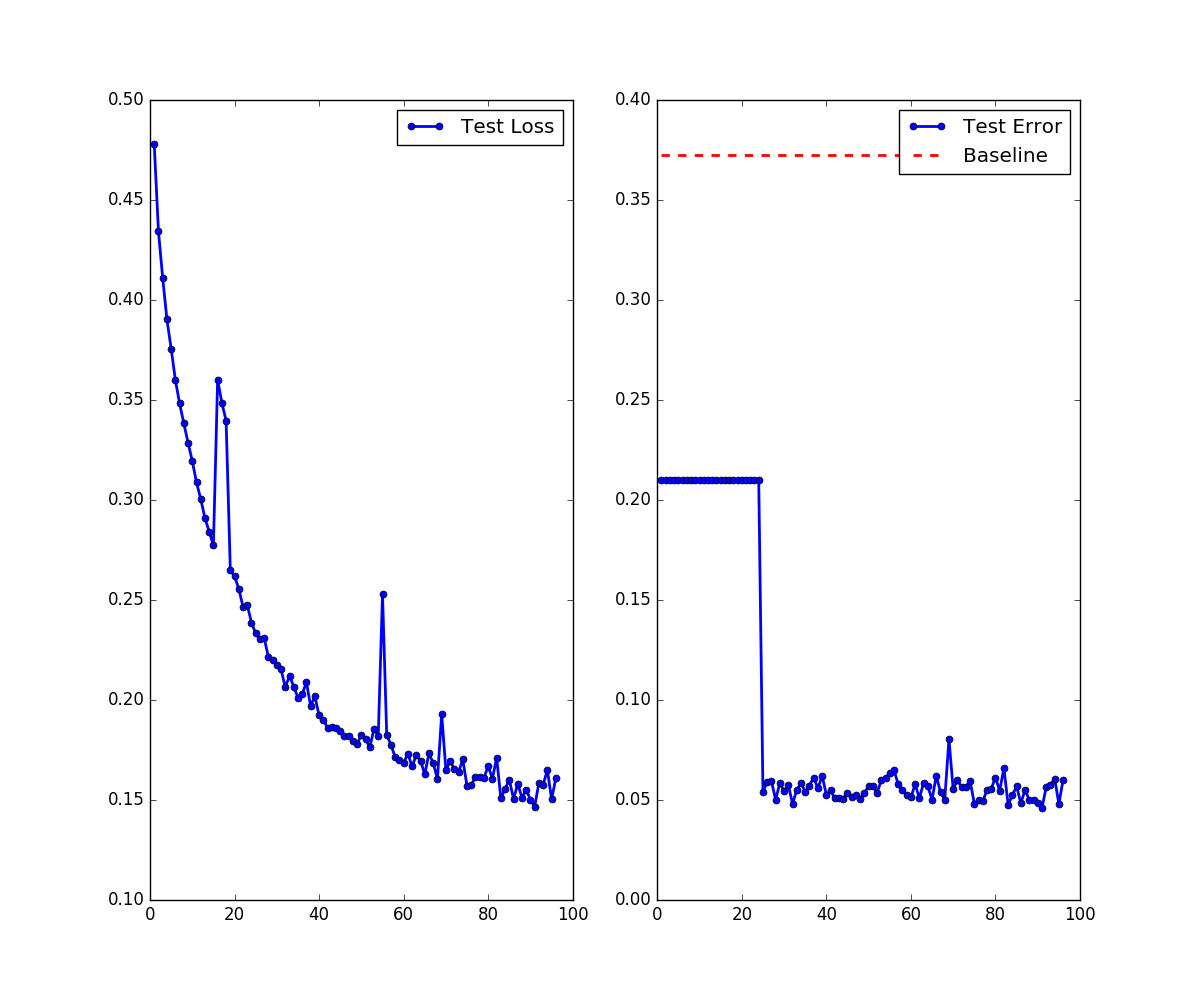
\includegraphics[width=0.95\textwidth]{Test-Statistics-sgd-batchsize=100-bce.png}
\end{minipage}
\end{figure}
\end{flushleft}

\subsection*{Part d}
\begin{flushleft}
Clearly, for the same learning rate and the same number of epochs, it would be hard to view similar performance. Hence, I change the learning rate (to 0.01) and train the network for a bit longer (2000 epochs). The final results after 96 iterations and the end of the training are reported below:
\begin{center}
\begin{tabular}{|c|c|c|}
\hline
& Train Accuracy & Test Accuracy \\
\hline
\hline
96 epochs & \(\approx 78\%\) & \(\approx 79\%\) \\
\hline
2000 epochs & \(93.11\%\) & \(94.27\%\) \\
\hline
\end{tabular}
\end{center}

The variation graph is shown below (L: Train, R: Test):
\begin{figure}[H]
\begin{minipage}{0.49\linewidth}
\centering
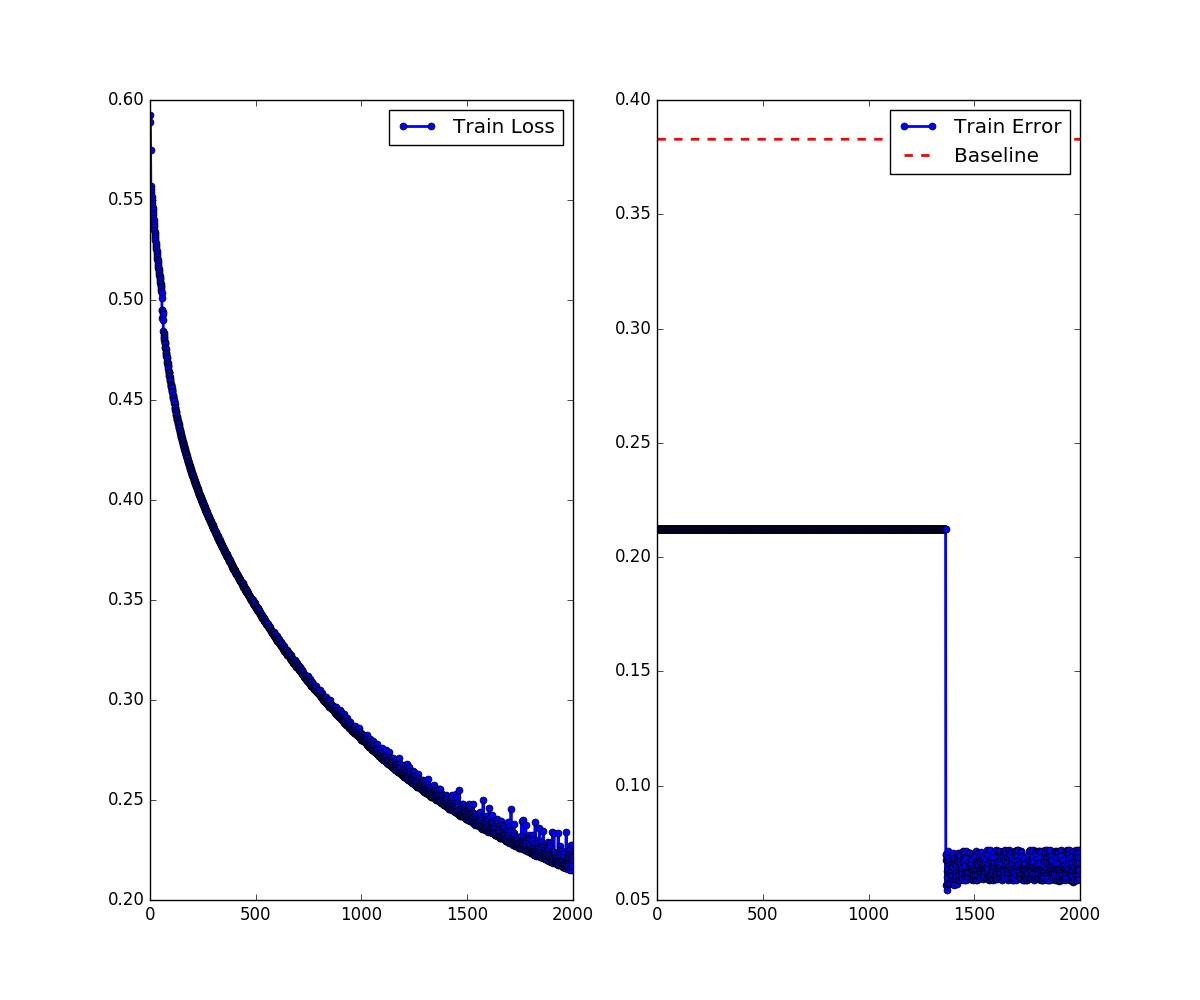
\includegraphics[width=0.95\textwidth]{Train-Statistics-sgd-batchsize=8143-bce.png}
\end{minipage}
\hfill
\begin{minipage}{0.49\linewidth}
\centering
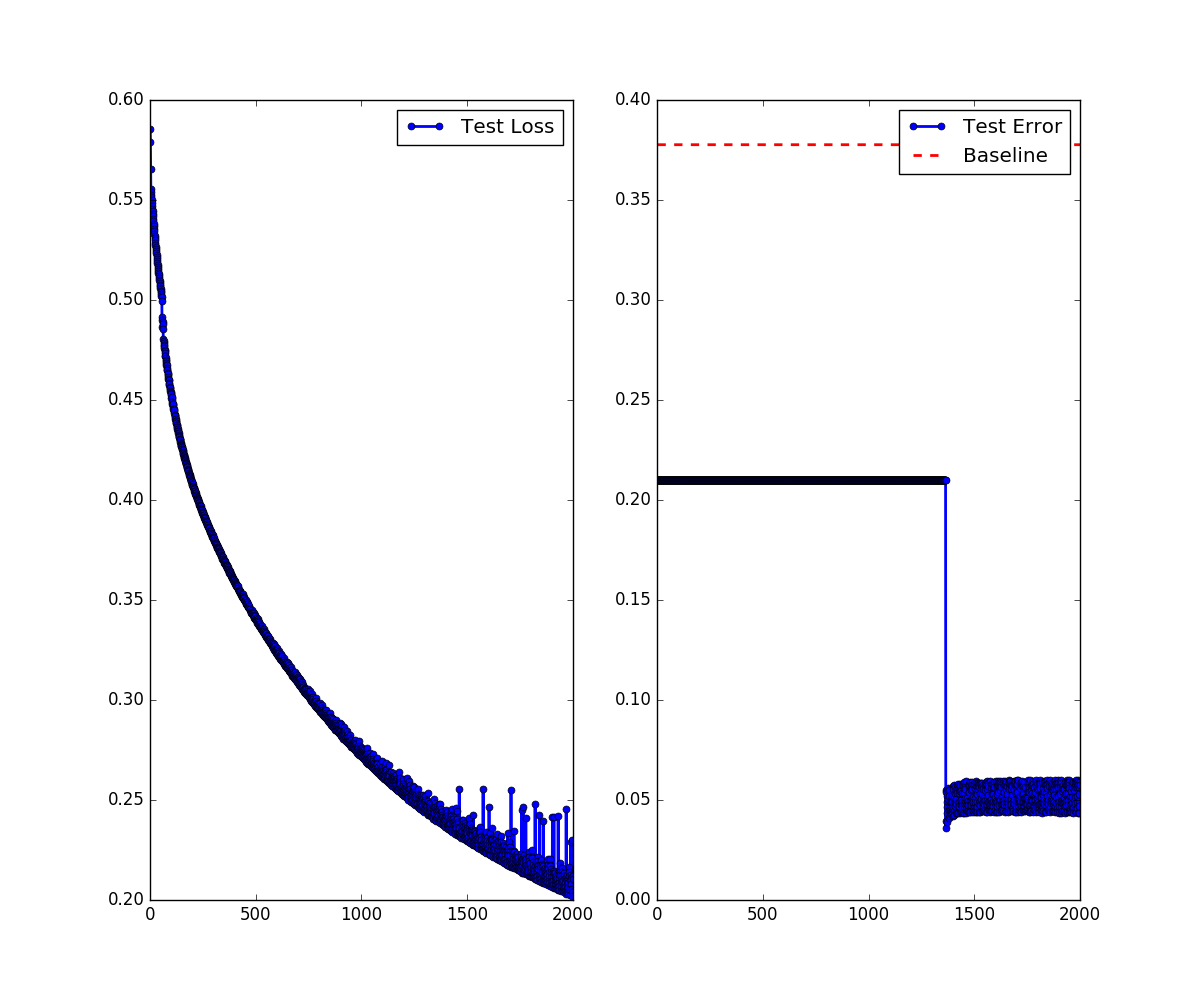
\includegraphics[width=0.95\textwidth]{Test-Statistics-sgd-batchsize=8143-bce.png}
\end{minipage}
\end{figure}
\end{flushleft}

\subsection*{Part e}
\begin{flushleft}
I use Adam as the learning algorithm for this sub-problem. The global learning rate in Adam is set to \(3 \times 10^{-4}\) (following Andrej Karpathy's claim), and the bias correction parameters are set to the default values. The stopping epochs for the 5 different configurations and the end performance are tabulated below:
\begin{center}
\begin{tabular}{|c|c|c|c|}
\hline
H & Stopping Epochs & Training Set Accuracy & Testing Set Accuracy \\
\hline
\hline
1 & 55 & \(\approx 78.6\%\) & \(\approx 79.1\%\)\\
\hline
2 & 350 & \(\approx 98.8\%\)& \(\approx 99.0\%\)\\
\hline
5 & 110 & \(\approx 98.8\%\)& \(\approx 99.1\%\)\\
\hline
10 & 90 & \(\approx 98.8\%\)& \(\approx 99.1\%\)\\
\hline
20 & 70 & \(\approx 98.8\%\)& \(\approx 99.2\%\)\\
\hline
\end{tabular}
\end{center}

Graphically, the variation is shown below (L: Train, R: Test):
\begin{minipage}{0.49\linewidth}
\begin{figure}[H]
\centering
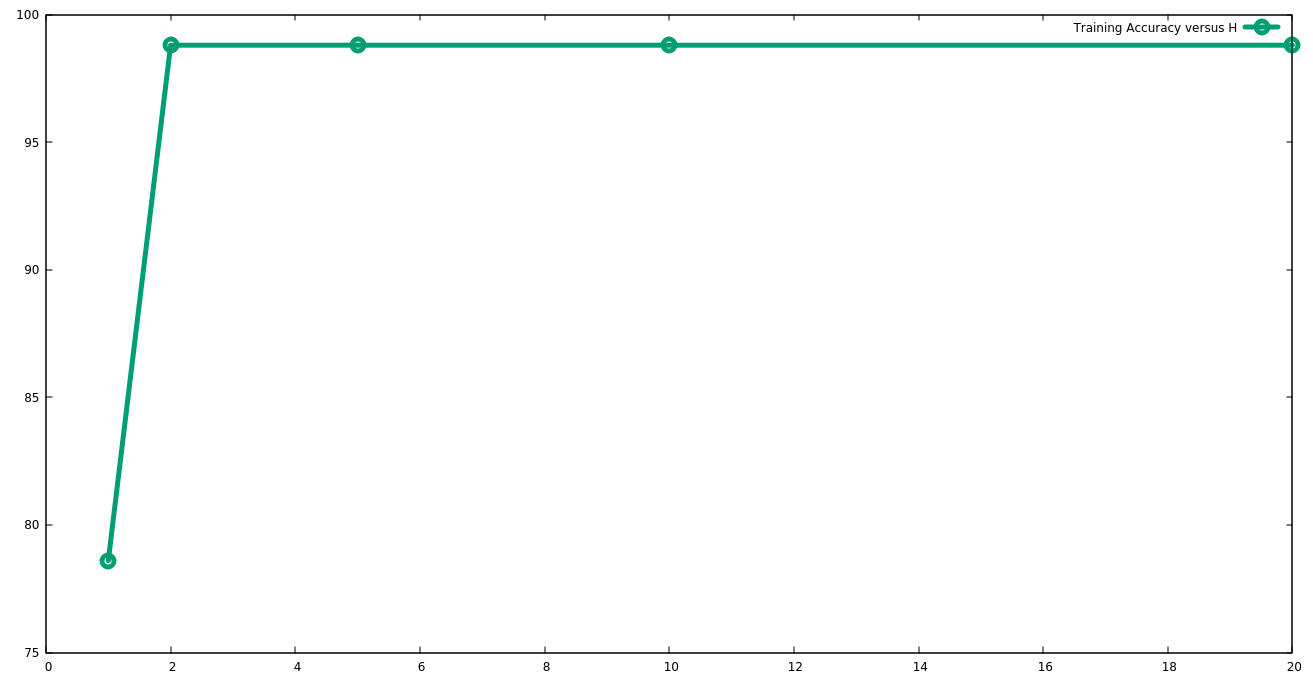
\includegraphics[width=0.95\textwidth]{train_H_BCE.png}
\end{figure}
\end{minipage}
\hfill
\begin{minipage}{0.49\linewidth}
\begin{figure}[H]
\centering
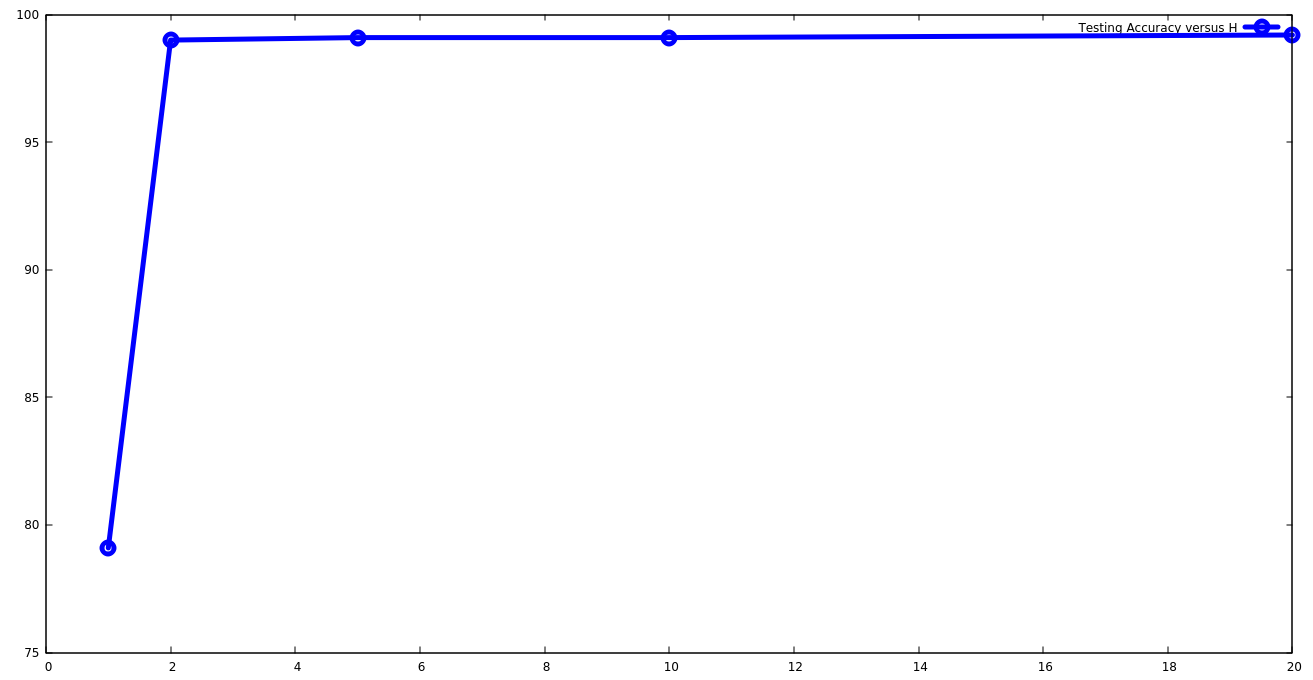
\includegraphics[width=0.95\textwidth]{test_H_BCE.png}
\end{figure}
\end{minipage}
\end{flushleft}

\subsection*{Part f}
\begin{flushleft}
The optimal learning chosen from the same set of specified above is 0.008. The training set accuracy achieved after 70 epochs was \(95\%\) and the testing set accuracy achieved after 70 epochs was \(\approx 96.1\%\). Below are the graphs of the variations observed (L: Train, R: Test):
\begin{figure}[H]
\begin{minipage}{0.49\linewidth}
\centering
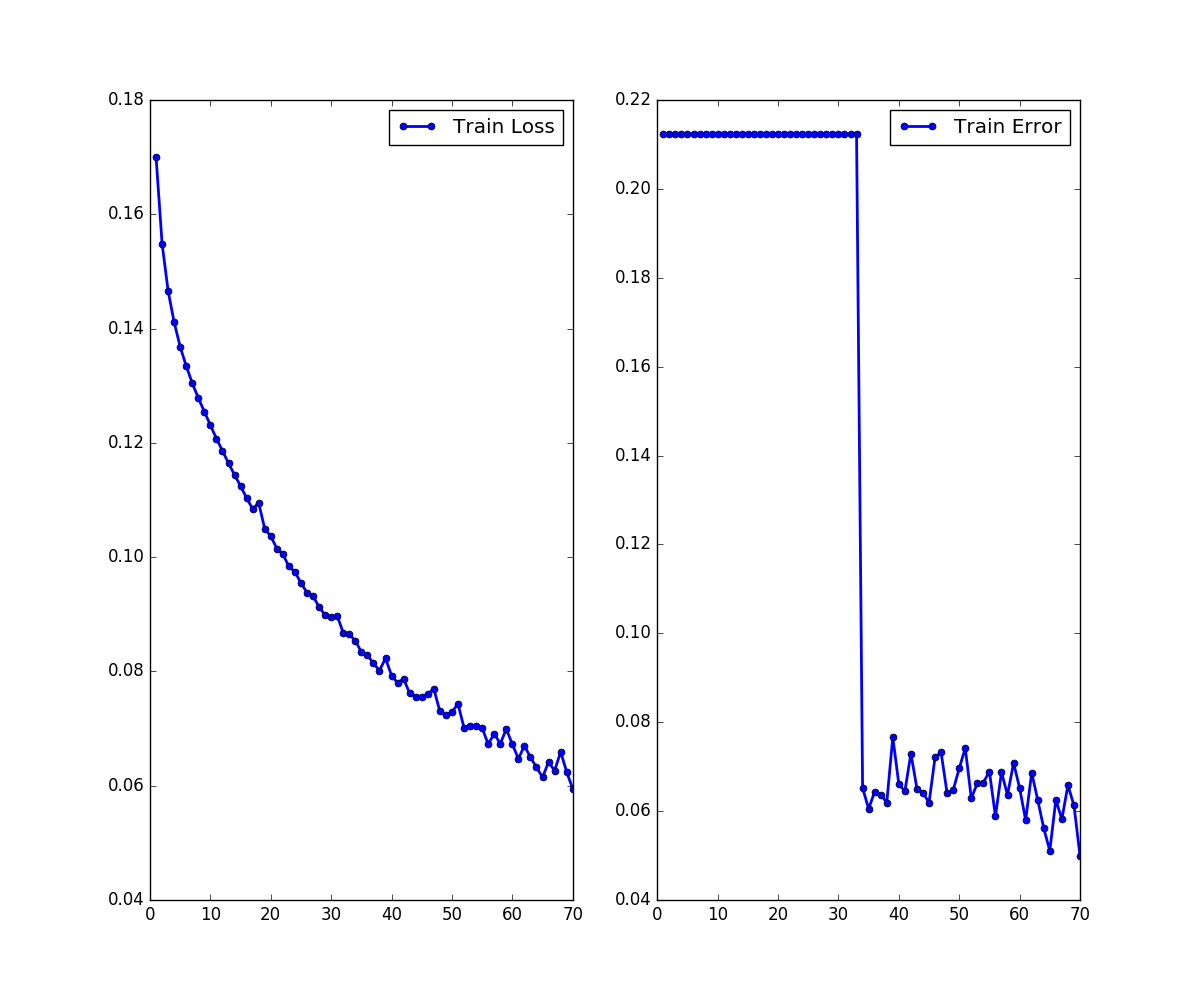
\includegraphics[width=0.95\textwidth]{Train-Statistics-sgd-batchsize=100-mse.png}
\end{minipage}
\hfill
\begin{minipage}{0.49\linewidth}
\centering
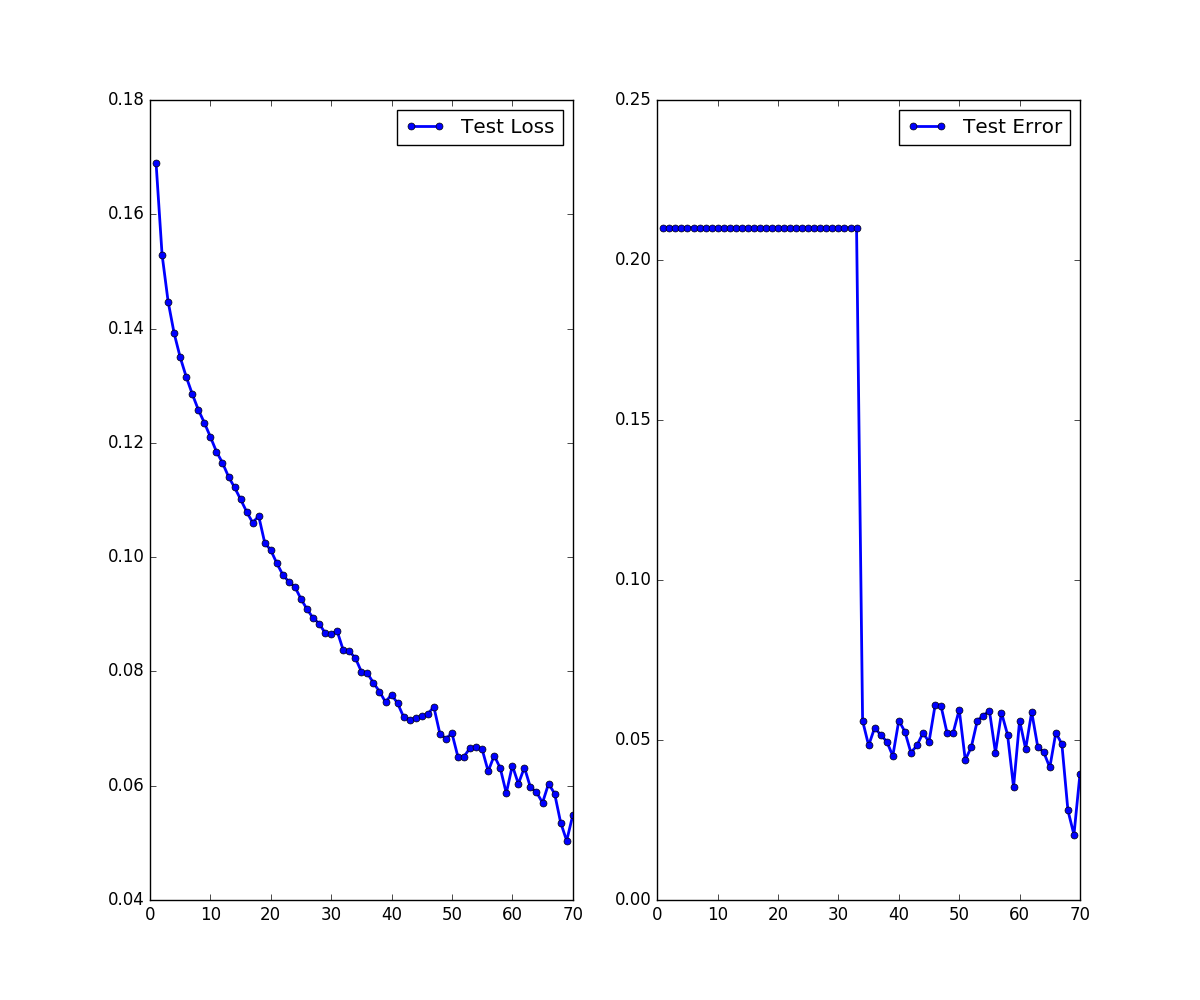
\includegraphics[width=0.95\textwidth]{Test-Statistics-sgd-batchsize=100-mse.png}
\end{minipage}
\end{figure}

In the full batch gradient descent, I run it for 3000 epochs. The results are graphed and tabulated below:
\begin{center}
\begin{tabular}{|c|c|c|}
\hline
& Train Accuracy & Test Accuracy \\
\hline
\hline
96 epochs & \(\approx 78.7\%\) & \(\approx 79.4\%\) \\
\hline
3000 epochs & \(94.4\%\) & \(97.99\%\) \\
\hline
\end{tabular}
\end{center}

The variation graph is shown below (L: Train, R: Test):
\begin{figure}[H]
\begin{minipage}{0.49\linewidth}
\centering
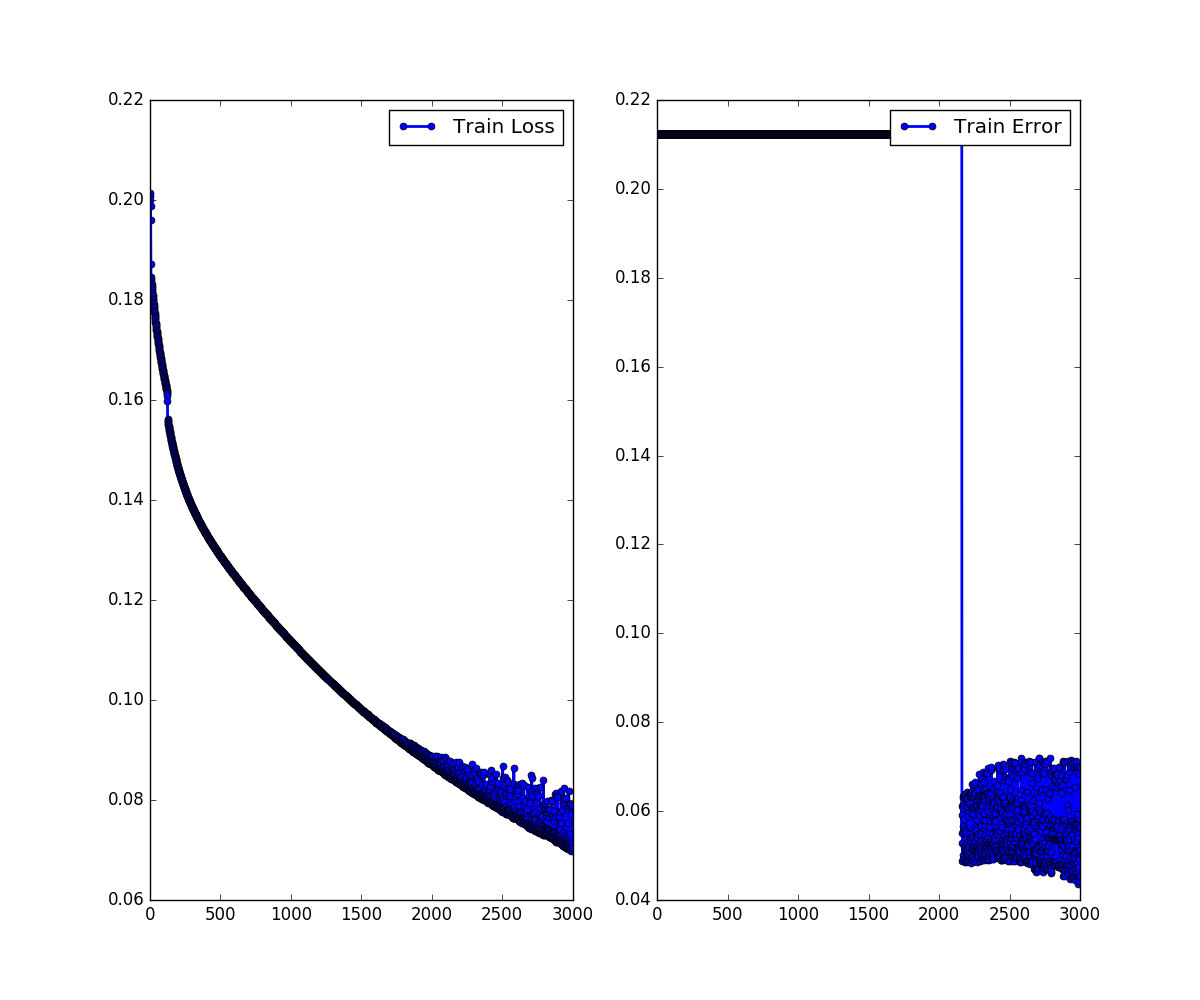
\includegraphics[width=0.95\textwidth]{Train-Statistics-sgd-batchsize=8143-mse.png}
\end{minipage}
\hfill
\begin{minipage}{0.49\linewidth}
\centering
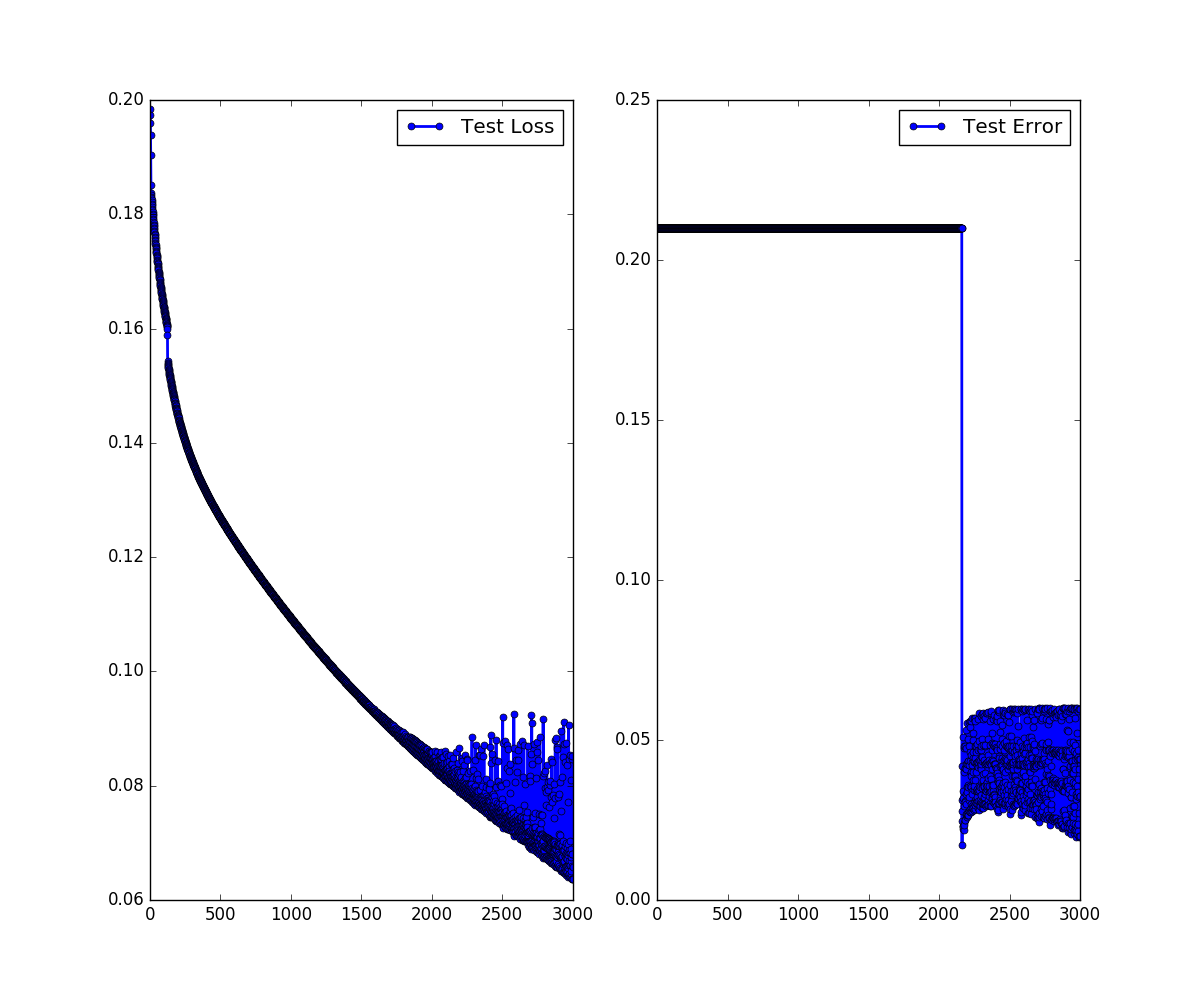
\includegraphics[width=0.95\textwidth]{Test-Statistics-sgd-batchsize=8143-mse.png}
\end{minipage}
\end{figure}

The stopping epochs for the 5 different configurations and the end performance are tabulated below for the analogue of the \textbf{Part e} for the Mean Squared Loss:
\begin{center}
\begin{tabular}{|c|c|c|c|}
\hline
H & Stopping Epochs & Training Set Accuracy & Testing Set Accuracy \\
\hline
\hline
1 & 55 & \(\approx 78.8\%\) & \(\approx 79.0\%\)\\
\hline
2 & 290 & \(\approx 98.8\%\)& \(\approx 99.2\%\)\\
\hline
5 & 110 & \(\approx 98.8\%\)& \(\approx 99.2\%\)\\
\hline
10 & 75 & \(\approx 98.8\%\)& \(\approx 99.3\%\)\\
\hline
20 & 65 & \(\approx 98.8\%\)& \(\approx 99.3\%\)\\
\hline
\end{tabular}
\end{center}

Graphically, the variation is shown below (L: Train, R: Test):
\begin{minipage}{0.49\linewidth}
\begin{figure}[H]
\centering
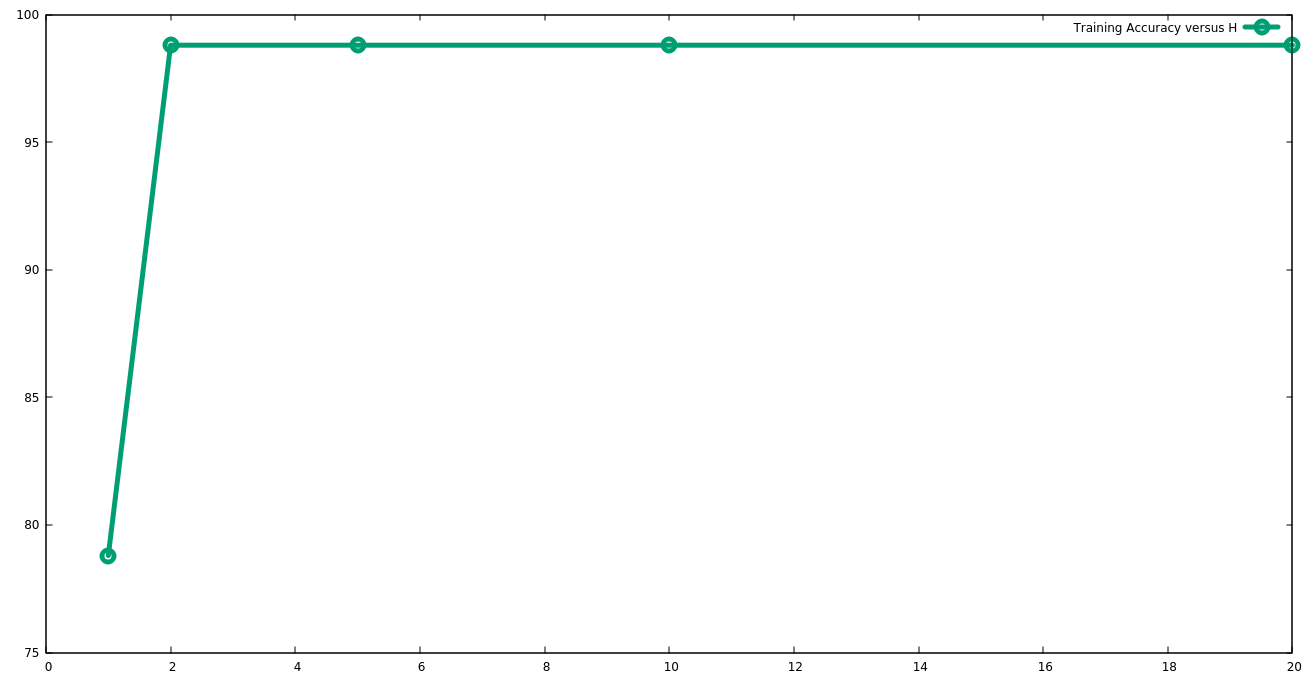
\includegraphics[width=0.95\textwidth]{train_H_MSE.png}
\end{figure}
\end{minipage}
\hfill
\begin{minipage}{0.49\linewidth}
\begin{figure}[H]
\centering
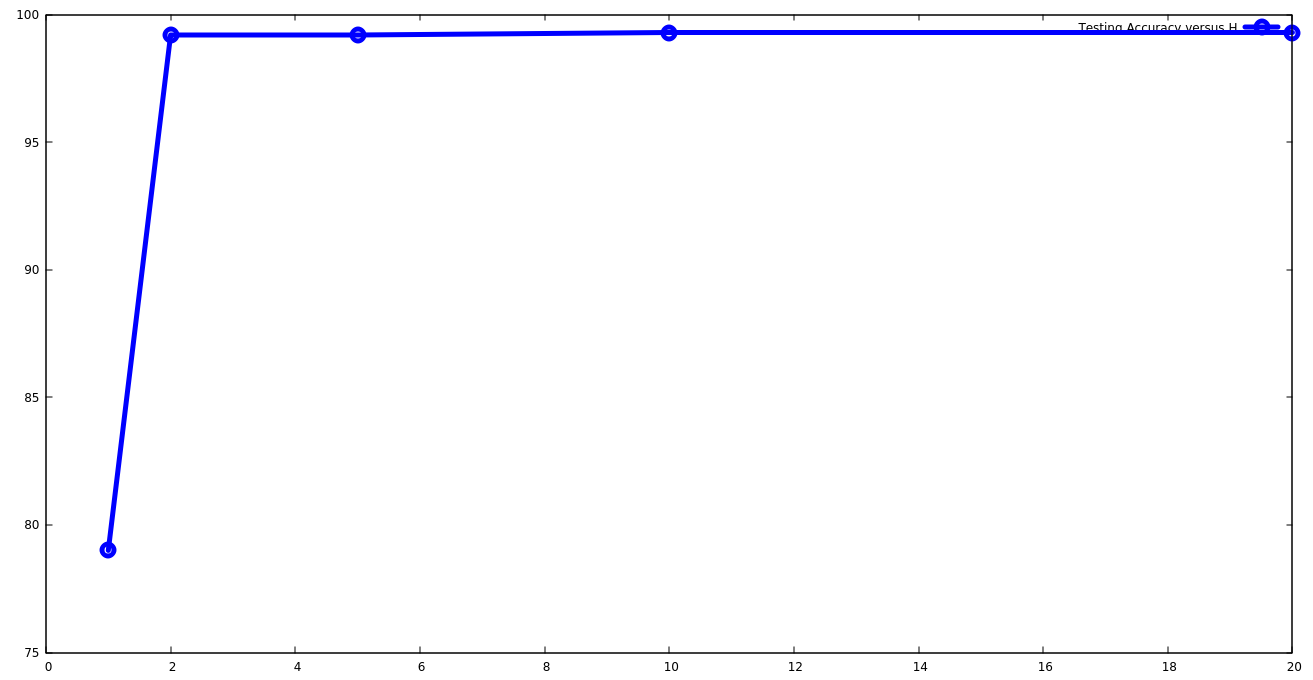
\includegraphics[width=0.95\textwidth]{test_H_MSE.png}
\end{figure}
\end{minipage}
\end{flushleft}

\subsection*{Part g}
\begin{flushleft}
The architecture, epochs trained for and the training and testing accuracies are tabulated below. The loss function is consideration is the binary-cross entropy loss.
\begin{center}
\begin{tabular}{|c|c|c|c|}
\hline
Architecture & Epochs Trained for & Training Accuracy & Testing Accuracy \\
\hline
\hline
\texttt{5 - 3 - 2 - 1} & 225 & \(\approx 98.9\%\) & \(\approx 98.1\%\)\\
\hline
\texttt{5 - 2 - 2 - 1} & 225 & \(\approx 98.9\%\) & \(\approx 99.1\%\)\\
\hline
\texttt{5 - 10 - 5 - 1} & 100 & \(\approx 98.9\%\) & \(\approx 98.9\%\)\\
\hline
\texttt{5 - 2 - 3 - 1} & 190 & \(\approx 98.9\%\) & \(\approx 99.1\%\)\\
\hline
\texttt{5 - 10 - 1} & 75 & \(\approx 98.8\%\) & \(\approx 99.2\%\)\\
\hline
\end{tabular}
\end{center}

From the table, it can be seen that multi-hidden-layer neural networks have a (little) better training accuracy than the single layer neural networks. Maybe, because of the over-parameterization, there is a reason of that very small dip in testing accuracy. I use the Adam Optimizer with a global learning rate of \(3 \times 10^{-4}\).
\end{flushleft}

\section*{Question 2}
The code for this question is in \texttt{Question2.py}. Please run \texttt{python3 Question2.py -h} for details and instructions.
\subsection*{Part a}
\begin{flushleft}
Below are the training and testing accuracies obtained while using \texttt{ReLU} and \texttt{Sigmoid}. The network was trained for 20 epochs, with a batch size of 64. The random state was set using the same obtained for the previous question (\texttt{random-state.pt}) to make the results comparable. The optimizer used was SGD with momentum (no Nesterov acceleration), with a momentum value of 0.9 and a learning rate of \(10^{-4}\).
\begin{center}
\begin{tabular}{|c|c|c|}
\hline
Activation & Training Accuracy & Testing Accuracy \\
\hline
\hline
\texttt{Sigmoid} & \(11.237\%\)& \(11.35\%\)\\
\hline
\texttt{ReLU} & \(94.615\%\) & \(94.85\%\)\\
\hline
\end{tabular}
\end{center}

However, while observing the variation of the training loss: it could be seen that the net with \texttt{Sigmoid} activation function was making progress, albeit slowly. The \texttt{ReLU} activation function was making steady and fast progress on the contrary. I believe that the reason for this could be two-fold:
\begin{itemize}
\item Initialization
\item Vanishing gradients problem due to the sigmoid function
\end{itemize}

The graph of the variation is shown below (L: \texttt{ReLU}, R: \texttt{Sigmoid}). Note the scale of the graph for the \texttt{Sigmoid}:
\begin{figure}[H]
\begin{minipage}{0.49\linewidth}
\centering
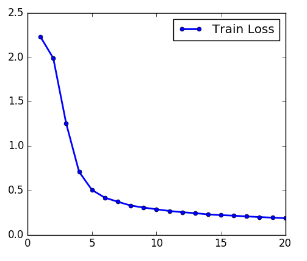
\includegraphics[width=0.9\textwidth]{train_loss_relu.png}
\end{minipage}
\hfill
\begin{minipage}{0.49\linewidth}
\centering
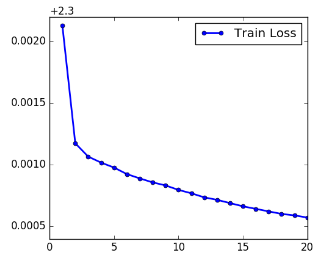
\includegraphics[width=0.9\textwidth]{train_loss_sigmoid.png}
\end{minipage}
\end{figure}
\end{flushleft}

\subsection*{Part b}
\begin{flushleft}
Intuitively, extremely high dropout could be detrimental to performance since nodes are zeroed out with a higher probability. But, dropout acts as a regularizer of sorts, hence there is an optimal value of dropout probability (that is not too high) that would give maximal testing accuracy. While running the experiments (no changes from the previous optimizer setup, except here I train for 50 epochs), this is what I observed:
\begin{center}
\begin{tabular}{|c|c|c|}
\hline
Dropout probability & Training Accuracy & Testing Accuracy\\
\hline
\hline
0.0 (No Dropout) & \(98.13\%\) & \(98.26\%\)\\
\hline
0.25 (1 in 4 nodes get dropped) & \(97.6\%\) & \(97.73\%\)\\
\hline
0.5 (1 in 2 nodes get dropped) & \(96.83\%\) & \(96.9\%\)\\
\hline
0.75 (3 in 4 nodes get dropped) & \(94.95\%\) & \(95.3\%\)\\
\hline
1.0 (All Dropout) & \(13.72\%\) & \(14\%\)\\
\hline
\end{tabular}
\end{center}

One change worth noticing is that the difference between the training accuracy and testing accuracy decreases with increasing dropout probability until 0.5. This indicates that the model is robust, but is just not as good as the model without dropout.
\end{flushleft}

\subsection*{Part c}
\begin{flushleft}
Below are the results for dropout and no dropout with batch normalization. I have considered the dropout probability to be 0.25 from the above table, and train the network for 50 epochs.
\begin{center}
\begin{tabular}{|c|c|c|}
\hline
Dropout present & Training Accuracy & Testing Accuracy\\
\hline
\hline
\texttt{True} & \(98.435\%\) & \(98.39\%\)\\
\hline
\texttt{False} & \(97.99\%\) & \(98.17\%\)\\
\hline
\end{tabular}
\end{center}

If you can compare the performance of all models with and without Dropout and Batch Normalization, you will be able to see that the model with Dropout and Batch normalization have performed the best. Below are the tabulated results:
\begin{center}
\begin{tabular}{|c|c|c|}
\hline
Model Type & Training Accuracy & Testing Accuracy\\
\hline
\hline
Without both Dropout and Batch Normalization & \(98.13\%\) & \(98.26\%\)\\
\hline
With only Dropout (p = 0.25) & \(97.6\%\) & \(97.73\%\)\\
\hline
With only Batch Normalization & \(97.99\%\) & \(98.17\%\)\\
\hline
With both Dropout and Batch Normalization & \(\mathbf{98.435}\%\) & \(\mathbf{98.39}\%\) \\
\hline
\end{tabular}
\end{center}
\end{flushleft}

\subsection*{Part d}
\begin{flushleft}
The different initialization strategies tried are: \emph{Xavier's Uniform Initialization}, \emph{Kaiming He's Uniform Initialization} and \emph{Default Initialization}.

The effects should be seen in the earlier stages of training, which is why I train for only 15 epochs with Batch Normalization. The results are tabulated below:
\begin{center}
\begin{tabular}{|c|c|c|}
\hline
Initialization & Training Accuracy & Testing Accuracy \\
\hline
\hline
Xavier & \(\mathbf{97.01}\%\) & \(\mathbf{97.15}\%\)\\
\hline
Kaiming & \(95.38\%\) & \(95.59\%\)\\
\hline
Default & \(96.49\%\) & \(96.88\%\)\\
\hline
\end{tabular}
\end{center}

From this, it should be evident that initialization plays a role in the result even with batch normalization. Below are the graphs for the variation of the training loss with the number of iterations (TopLeft: \emph{Xavier}, TopRight: \emph{Kaiming}, BottomCenter: \emph{Default}).
\begin{figure}[H]
\begin{minipage}{0.49\linewidth}
\centering
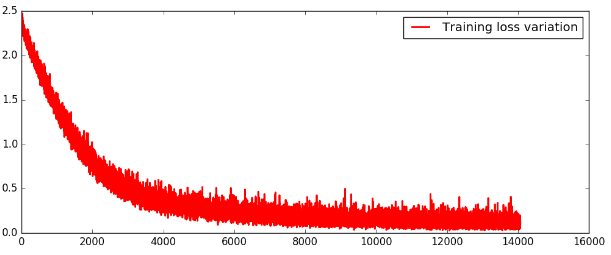
\includegraphics[width=\textwidth]{xavier_init.png}
\end{minipage}
\hfill
\begin{minipage}{0.49\linewidth}
\centering
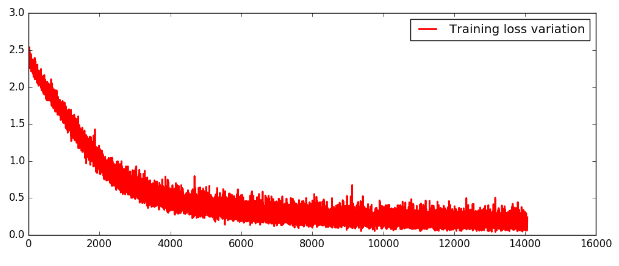
\includegraphics[width=\textwidth]{kaiming_init.png}
\end{minipage}
\end{figure}

\begin{figure}[H]
\centering
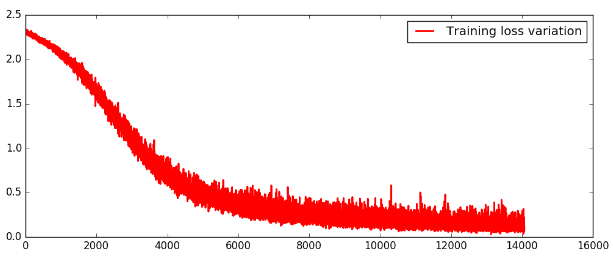
\includegraphics[width=0.485\linewidth]{default_init.png}
\end{figure}

In the beginning 2 epochs, I believe that SGD with momentum performed better with Xavier's init than the others. After that, the behaviour is very similar.
\end{flushleft}
\end{document}
